\documentclass{standalone}

\begin{document}


\section*{FiloBlu Service}\addcontentsline{toc}{section}{FiloBlu Service}
\markboth{Appendix E}{FiloBlus Service}

In the \emph{FiloBlu} project we have a stream of data provided by an external APP that are stored in a central database server.
The Machine Learning service has to read the information stored into a database, it processes them and finally it writes the results into the same database.
All these operations have to be performed with high frequency since the output results have to be shown in a real-time application.
This frequency would be the clock-time of the process function, i.e at each time interval (as small as we like) the process task will be called and we will have the desired results in output.
At the same time we have to take care about the time required by our Machine Learning algorithm: not all the algorithms can process data in real time and the frequency of process function has to be less than the time required by the algorithm or we can loose some information.

We obtain the best efficiency from a service splitting as much as possible the required functionality in small-and-easy tasks.
Small tasks can be evaluated as independent functions with an associated frequency that in this case can be reduced as much as possible.
The \emph{FiloBlu} functionalities can be reviewed as a sequence of 3 fundamental steps and other 2 optional ones: 1) read the data from the database, 2) process the data with the Machine Learning algorithm and 3) write the obtained results into the database; 4) update the Machine Learning model and 5) clear old log files are optional steps.
To further improve the service efficiency we give each (independent) step to a different thread.
The whole set of tasks are piloted by a master thread given by the service itself.
In this way the service is computational efficient and moreover it does not weight on the computer performances.
We have to take in mind that the computer which hosts the service has to be affected by the daemon process as less as possible either in memory either on computational efficiency.
The last step is the synchronization of the previous tasks with appropriate clock frequencies.

Let's start from the data reading function.
Since our data are assumed to be stored into a database, this function has to perform a simple query and extract the latest data inserted.
Obviously the efficiency of the step is based on the efficiency of the chosen query.
The data extracted are saved in a common container shared between the list of threads and thus it belongs to the master.
The choice of an appropriate container is a second point to carefully takes in mind.
This container should be light an thread-safe to avoid thread concurrency.
While the second request is implementation dependent, the first one can be faced on using a \textsf{FIFO} container\footnote{
  FIFO container, i.e \emph{First-In-First-Out}, is a special data structure in which the first element added will be processed as first and then automatically removed from it.
}.
In this way we can ensure that the application will save a fixed amount of data and it will not occupy large portion of memory (RAM).

The second task is identified by the Machine Learning function which processes the data.
The algorithm takes the data from the \textsf{FIFO} container of the previous step (if there are) and it saves the results into a second \textsf{FIFO} container for the next step.
The time frequency of the step is given by the time required by the Machine Learning algorithm.

The third step takes the data from the second \textsf{FIFO} container (if there are) and it performs a second query (a writing one in this case) to the database.
Also in this case the frequency is given by the efficiency of the chosen query.

The last two steps can be executed without time requirements and they are useful only on a large time scale.

Each step performs its independent logging on a single shared file.
If an error occurs the service logs an appropriate message and it saves the current log-file in a different location to prevent possible log-cleaning (optional step).
Then the service restarts.

\begin{figure}[htbp]
\centering
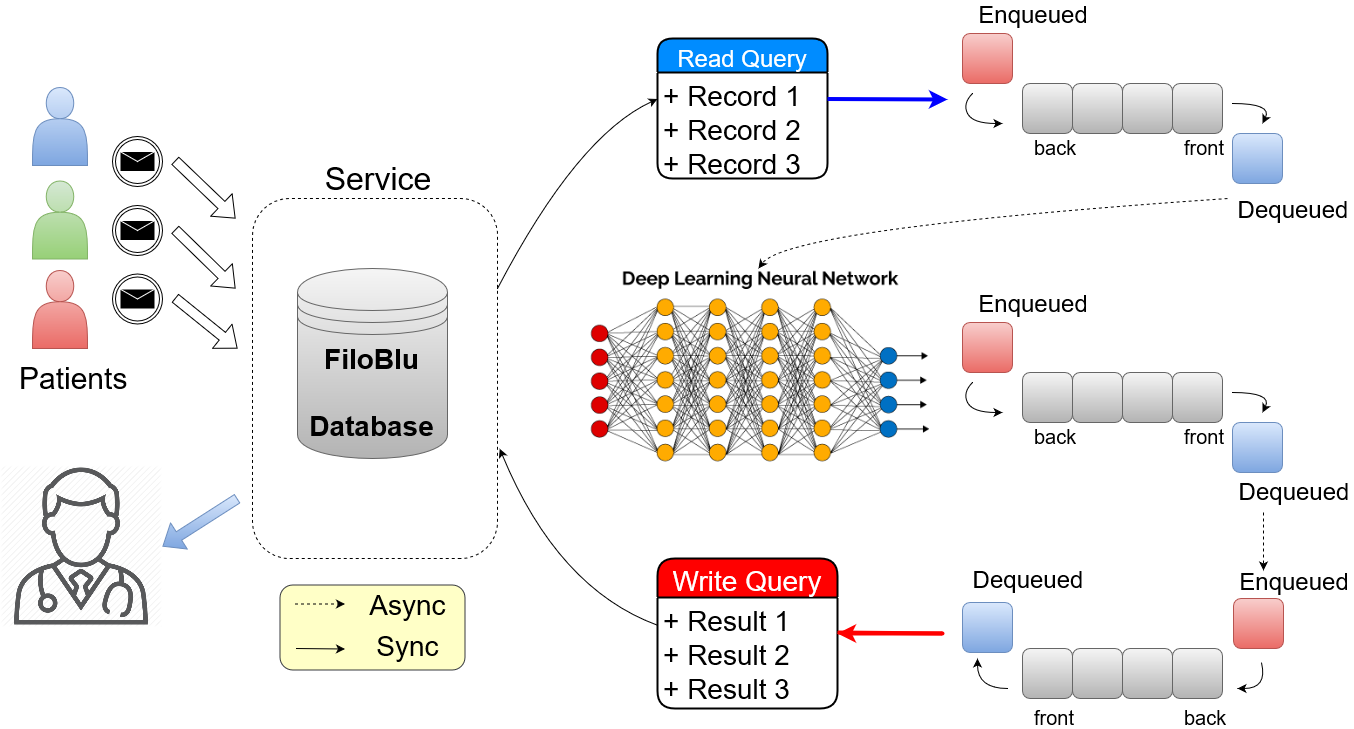
\includegraphics[width=.9\linewidth]{FiloBluService.png}
\caption{FiloBlu Service computation scheme.
}
\label{fig:FiloBlu}
\end{figure}

We implemented this type of service in pure \textsf{Python} and the code is publicly available on Github~\cite{FiloBlu}.
The developed service was customized according to the server requirements of the project\footnote{
  The FiloBlu service is a Windows service and it can not run on Unix machines.
  Moreover, the database used in the project is a \textsf{MySQL} one so the queries and the libraries used are compatible only with this kind of database.
}.
We chose the \textsf{Python} language either for its simplicity in the code writing either for its thread native module, which ensures a total thread-safety of each variable.
Using a set of function decorators we are able to run each function (\textsf{callback}) in a separated-detached thread as required by the previous instructions.
The project includes a documentation about its usage (also for general applications) and it can be easily installed via \href{https://github.com/Nico-Curti/FiloBluService/blob/master/setup.py}{\textsf{setup.py}}.
In the \emph{FiloBlu} project we used a Neural Network algorithm written in \textsf{Tensorflow} as Machine Learning model.
\textsf{Tensorflow} does not allow to run background processes directly, so the problem was overcame using a direct call to a \textsf{Python} script which performed the full list of steps into an infinite loop.
In this way the service could be restarted also if the process-service was killed.
The service can be driven using a simple \href{https://github.com/Nico-Curti/FiloBluService/blob/master/filobluservice.ps1}{\textsf{Powershell}} script provided in the project.

\end{document}
